\hypertarget{haskell}{%
\section{Haskell - Types}\label{haskell}}

Haskell has some basic types, including:

\begin{itemize}
\tightlist
\item
  Bool
\item
  Char
\item
  String
\item
  Int (fixed-precision integers)
\item
  Integer (arbitrary-precision integers)
\item
  Float
\end{itemize}

A list is sequence of values of the same type.

\hypertarget{tuple-types}{%
\subsubsection{Tuple Types}\label{tuple-types}}

A tuple is a sequence of values of different types.

\begin{lstlisting}[language=Haskell]
(False,'a',True) :: (Bool,Char,Bool)
ghci> fst (8,11)  
8  
ghci> snd (8,11)
11
\end{lstlisting}

In difference to the normal type of an array is the type of a tuple
encoding its size.

\hypertarget{function-types}{%
\subsection{Function Types}\label{function-types}}

A function is a mapping from values of one type to values of another type. Functions also have types. When writing our own functions, we can choose to give them an explicit type declaration. This is generally considered to be good practice except when writing very short functions.

\begin{lstlisting}[language=Haskell]
-- "::" is read as "has type of"
not :: Bool -> Bool

removeNonUppercase :: [Char] -> [Char]  
removeNonUppercase st = [ c | c <- st, c `elem` ['A'..'Z']]  
-- meaning that it maps from a string to a string. That's because it takes one string as a parameter and returns another as a result

addThree :: Int -> Int -> Int -> Int  
addThree x y z = x + y + z 
-- The parameters are separated with -> and there's no special distinction between the parameters and the return type.
\end{lstlisting}

\clearpage

\hypertarget{polymorphic-functions}{%
\subsubsection{Polymorphic Functions}\label{polymorphic-functions}}

A function is called polymorphic (``of many forms'') if its type
contains one or more type variables.

\begin{lstlisting}[language=Haskell]
For any type a, length takes a list of values of type a and returns an integer.
\end{lstlisting}

\hypertarget{overloaded-functions}{%
\subsubsection{Overloaded Functions}\label{overloaded-functions}}

A polymorphic function is called overloaded if its type contains one or
more class constraints.

\begin{tcolorbox}[colback=red!5!white,colframe=red!75!black]
For any numeric type a, (+) takes two values of type a and returns a value of type a.
\end{tcolorbox}

\subsection{Type variables}

\begin{lstlisting}[language=Haskell]
ghci> :t head  
head :: [a] -> a

ghci> :t fst  
fst :: (a, b) -> a  
\end{lstlisting}

Types are written in capital case, so it can't exactly be a type. Because it's not in capital case it's actually a type variable. That means that a can be of any type. This is much like generics in other languages, only in Haskell it's much more powerful because it allows us to easily write very general functions if they don't use any specific behavior of the types in them. Functions that have type variables are called polymorphic functions. The type declaration of head states that it takes a list of any type and returns one element of that type.

\clearpage
\subsection{Typeclasses}

If a type is a part of a typeclass, that means that it supports and implements the behavior the typeclass describes.

\begin{lstlisting}[language=Haskell]
ghci> :t (==)  
(==) :: (Eq a) => a -> a -> Bool  
\end{lstlisting}

We see a new thing here, the => symbol. Everything before the => symbol is called a class constraint. We can read the previous type declaration like this: the equality function takes any two values that are of the same type and returns a Bool. The type of those two values must be a member of the Eq class.

\begin{lstlisting}[language=Haskell]
ghci> :t (>)  
(>) :: (Ord a) => a -> a -> Bool 
\end{lstlisting}

Ord is for types that have an ordering. 

\subsection{Operation on Lists}
\label{sec:Operationonlists}
\begin{figure}[H]
\centering
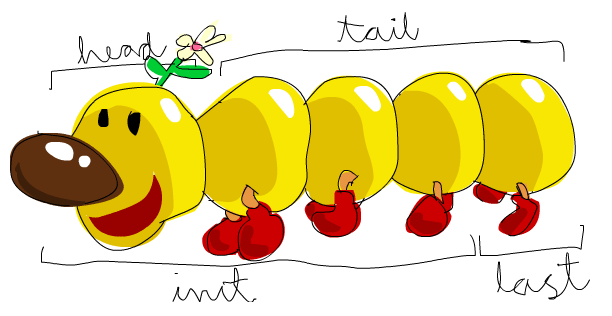
\includegraphics[width=0.5\textwidth]{figures/listOperations.png}
\caption{List operations}
\end{figure}

\begin{lstlisting}[language=Haskell]
ghci> [3,2,1] > [2,1,0]  
True  
ghci> [3,4,2] > [3,4]  
True
ghci> length [5,4,3,2,1]  
5
ghci> null [1,2,3]  
False 
ghci> reverse [5,4,3,2,1]  
[1,2,3,4,5] 
ghci> take 3 [5,4,3,2,1]  
[5,4,3]
ghci> drop 3 [8,4,2,1,5,6]  
[1,5,6] 
ghci> maximum [1,9,2,3,4]  
9  
ghci> sum [5,2,1,6,3,2,5,7]  
31
ghci> 4 `elem` [3,4,5,6]  
True 
ghci> ['a'..'z']  
"abcdefghijklmnopqrstuvwxyz"
ghci> [3,6..20]  
[3,6,9,12,15,18]
take 10 (cycle [1,2,3])  
[1,2,3,1,2,3,1,2,3,1]  
take 10 (repeat 5)  
[5,5,5,5,5,5,5,5,5,5]  
\end{lstlisting}

\clearpage